%====================================================================================================
% ?????
%====================================================================================================
% TCC
%----------------------------------------------------------------------------------------------------
% Autor				: Jasane Schio
% Orientador		: Gedson Faria
% Co-Orientador		: Angelo Darcy
% Instituição 		: UFMS - Universidade Federal do Mato Grosso do Sul
% Departamento		: CPCX - Sistema de Informação
%----------------------------------------------------------------------------------------------------
% Data de criação	: 01 de Outubro de 2015
%====================================================================================================
% 
\chapter{Testes e Resultados} 
Este capitulo será dividio em duas seções: \textbf{Calibração} e \textbf{Testes}. A seção \textbf{Calibração} tera a descrição do processo de calibração de cores, a preparação do campo, configuração de imagem, etc. A seção \textbf{Testes} é onde descrevo o testes usados para a análise de eficiência do sistema desenvolvido.
\section{Calibração}
A calibração aqui descrita ocorreu dia no 19 de Agosto de 2016, entre 17:36 e 17:39.
A rotina de calibração do sistema, já descrita no Capitulo 3 deste trabalho, envolve primeiramente uma aquisição da imagem do campo vazio, sem nada no mesmo, como visto na Figura \ref{campovazio}.
\begin{figure}[H]
		\centering
		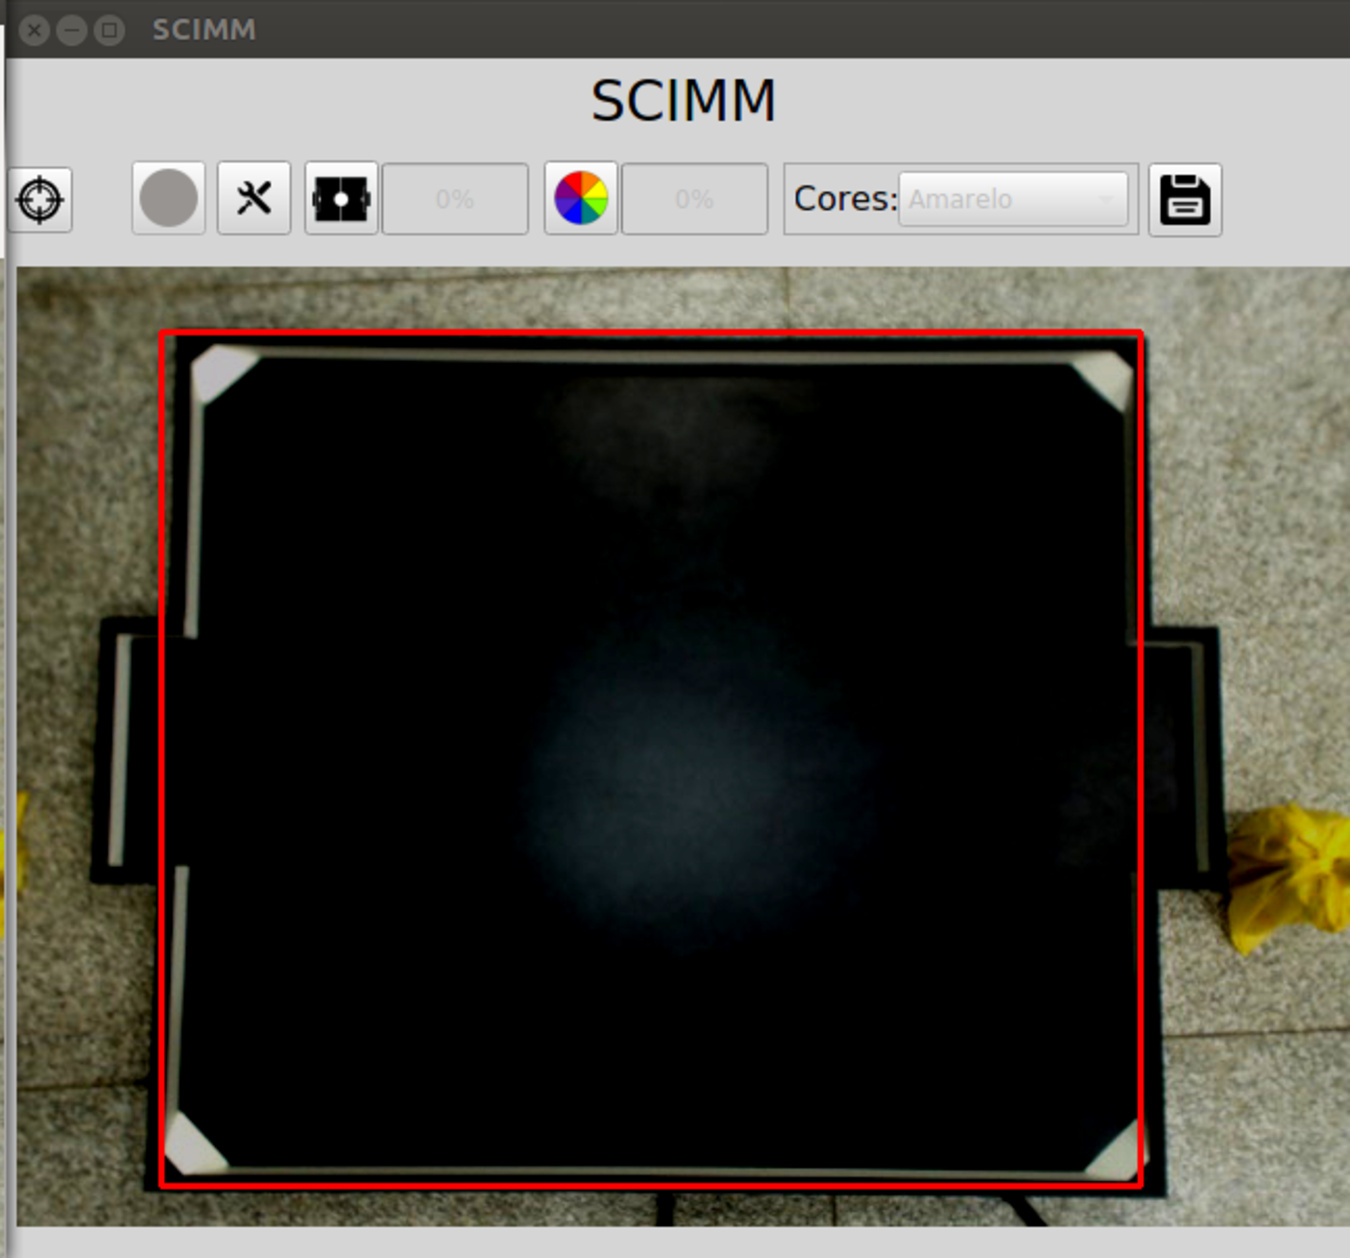
\includegraphics[width=0.45\textwidth]{fundoteste.pdf}
		\caption{Imagem do fundo com a seleção de campo}
		\label{campovazio}
	\end{figure}
Após ter o campo identificado pelo sistema, deve-se dispor sobre o campos os objetos coloridos, com as cores cujo se deseja obter o intervalo. É preferido que se usem tiras coloridas em vez de quadrado, de \textit{4cm x 4cm} como é comumente feito. Essa preferência se dá pois quanto maior o tamanho da tira de cor, maior sera o espectro de cores que seja analisado, assim sendo possível uma melhor qualidade de calibração.
Neste teste foram dispostos no campo tiras coloridas com largura entre \textit{17cm} e \textit{40cm} e altura entre \textit{5,5cm} e \textit{10,5cm}, cada cor com 3 tiras uma vez que o campo foi separado em três partes, significando as partes com diferentes luminosidades, sendo assim cada uma das tiras colocada em uma das partes do campos, como é possível visualiar na Figura \ref{fig:objetodispostos}.
	
	\begin{figure}[H]
%\begin{minipage}[H]{0.34\linewidth}
%\hspace{0.5cm}
\centering
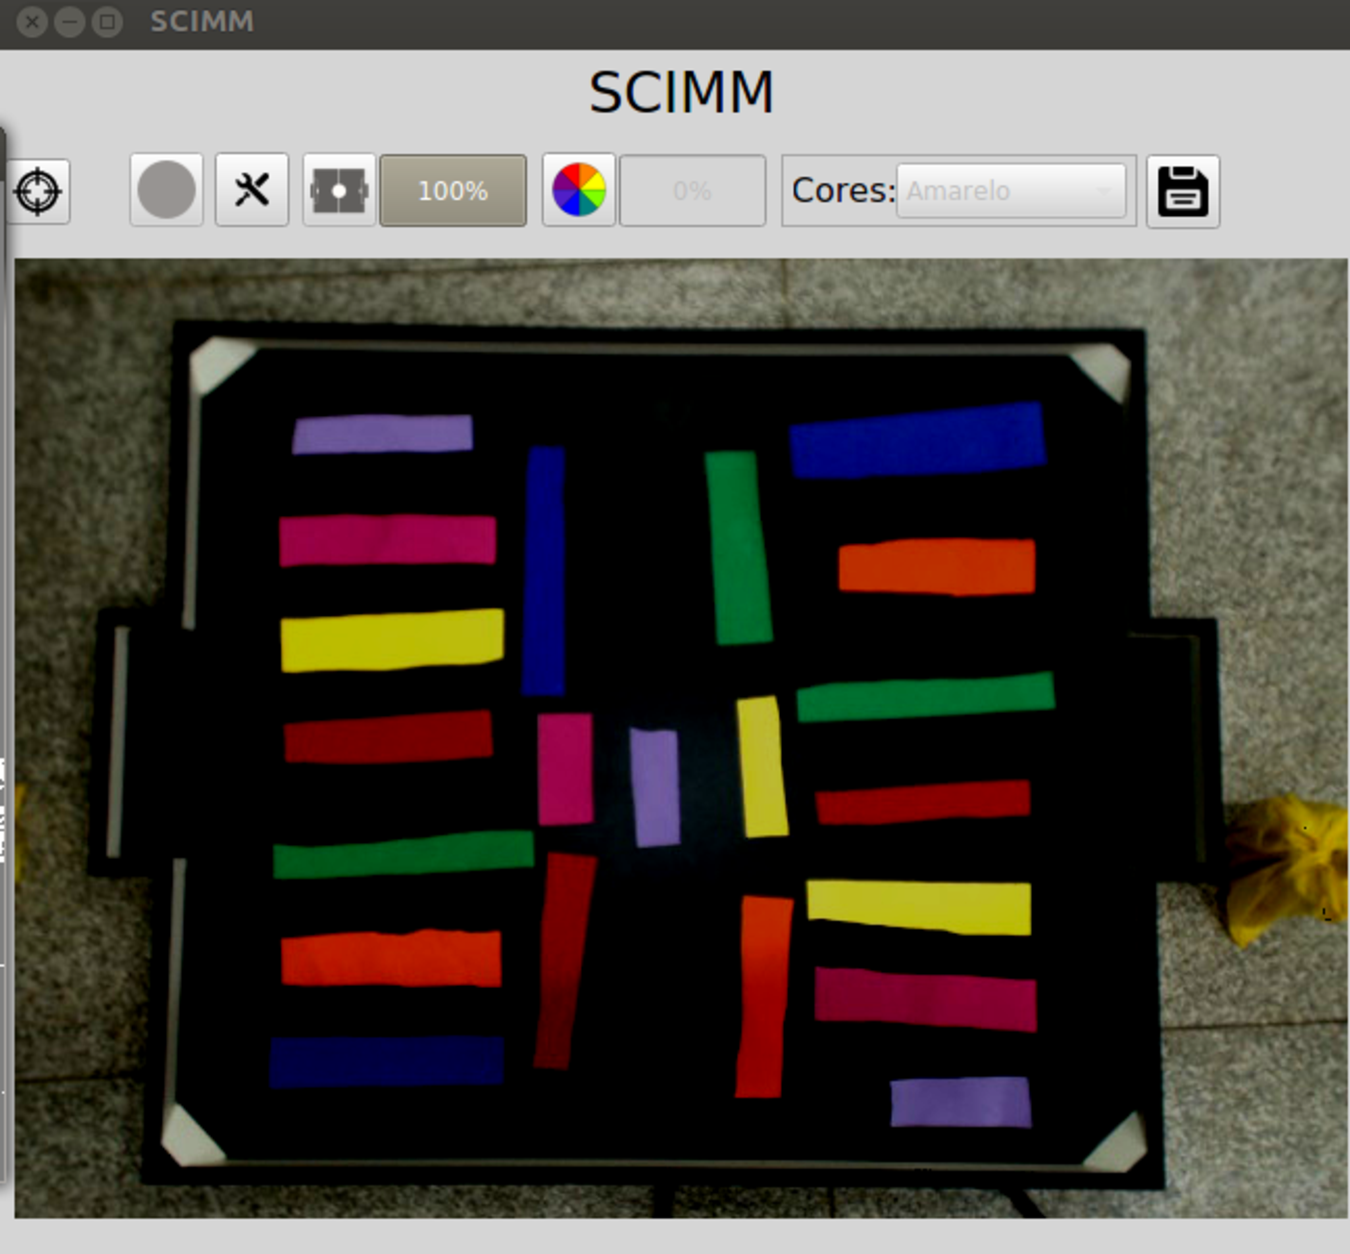
\includegraphics[width=0.45\textwidth]{objetosdispostos.pdf}
\caption{Objetos dispostos no campo para calibração}
\label{fig:objetodispostos}
%\end{minipage}
%\hspace{0.5cm}
%\begin{minipage}[H]{0.40\linewidth}
%\centering
%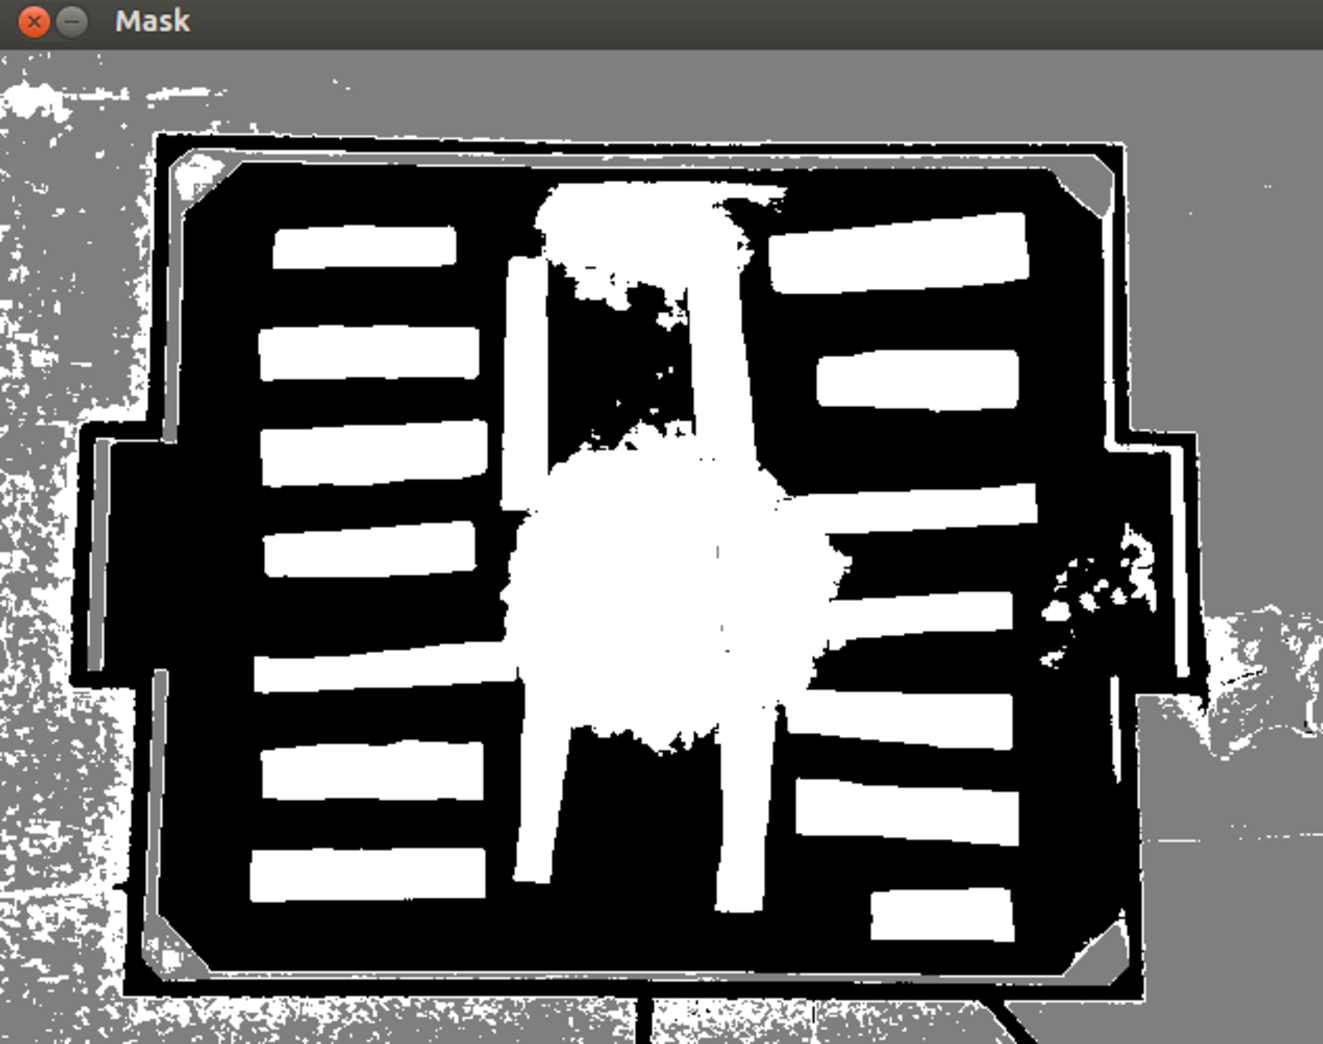
\includegraphics[width=\textwidth]{mascaragerada.pdf}
%\caption{Mascara gerada a partir da subtração de fundo}
%\label{fig:mascaragerada}
%\end{minipage}
\end{figure}	
	
Como resultado da rotina de calibraç\~{a}o foi gerado um arquivo .arff contendo 14 linhas. A tabela abaixo possui uma explicação sobre o arquivo gerado. A primeira coluna da tabela designa a linha contida no arquivo, a segunda coluna possui o conteúdo existente na linha do arquivo e na ultima coluna está a descrição do conteúdo do arquivo.
	\begin{table}[H]
\centering 
\begin{tabular}{l|c|c}
Linha & Conteúdo & Descrição  \\% Note a separação de col. e a quebra de linhas
\hline                               % para uma linha horizontal
 1& 21.50.50  &   Valor mínimo da cor Amarelo \\ \hline  
2& 30.255.255  &  Valor máximo da cor Amarelo \\  \hline 
3& 92.100.100  &   Valor mínimo da cor Azul \\  \hline 
4& 120.255.255  &  Valor máximo da cor  Azul \\  \hline 
5& 62.30.100 &  Valor mínimo da cor Verde \\  \hline 
6& 90.255.255  &  Valor máximo da cor Verde \\  \hline 
7& 169.100.100  &  Valor mínimo da cor Vermelho \\  \hline 
8& 179.255.255  &  Valor máximo da cor Vermelho \\   \hline 
9& 0.100.100  &  Valor mínimo da cor Laranja \\  \hline 
10& 20.255.255 &  Valor máximo da cor  Laranja \\  \hline 
11& 161.100.100 &  Valor mínimo da cor Rosa \\  \hline 
12& 168.255.255 &   Valor máximo da cor Rosa \\  \hline 
13& 126.30.30 &  Valor mínimo da cor Roxo \\  \hline 
14& 160.255.255 &  Valor máximo da cor Roxo \\  \hline 

\end{tabular}
\caption{Os valores de HSV est\~{a}o separados por pontuação, H.S.V}
\end{table}





 \section{Testes}
O teste aqui descrito ocorreu dia no 26 de Agosto de 2016, entre à 13:28 e 16:28.
Para elaboração do teste optou-se por dividir o campos no maior numero de partes possiveis, e ainda assim que essas partes coubessem todas as 7 cores usadas. Essa divisão foi feita para simular as cores em todas as partes possiveis do campos. O campo foi divido então em 15 partes de \textit{29cm} por \textit{41cm}, nomeadas alfabeticamente de A à O, como mostrado na Figura \ref{campodivisao}.

\begin{figure}[H]
		\centering
		\includegraphics[width=0.3\textwidth]{campodivisao.pdf}
		\caption{Divisão do campo em quinze partes nomeadas alfabeticamente.}
		\label{campodivisao}
	\end{figure}
	
Em cada uma das partes do campo estavam dispostas sete cores. Vermelho, Amarelo e Azul na primeira linha. Verde, Roxo, Laranja e Rosa na segunda. As cores estão distantes verticalmente \textit{6cm}, na primeria linha a distância entre as cores é de \textit{7,25cm} e na segunda linha de \textit{5cm}. Um  melhor detalhamento da disposição das cores é mostrado na Figura \ref{disposicaoparte}.


\begin{figure}[H]
\begin{minipage}[b]{0.45\linewidth}
\centering
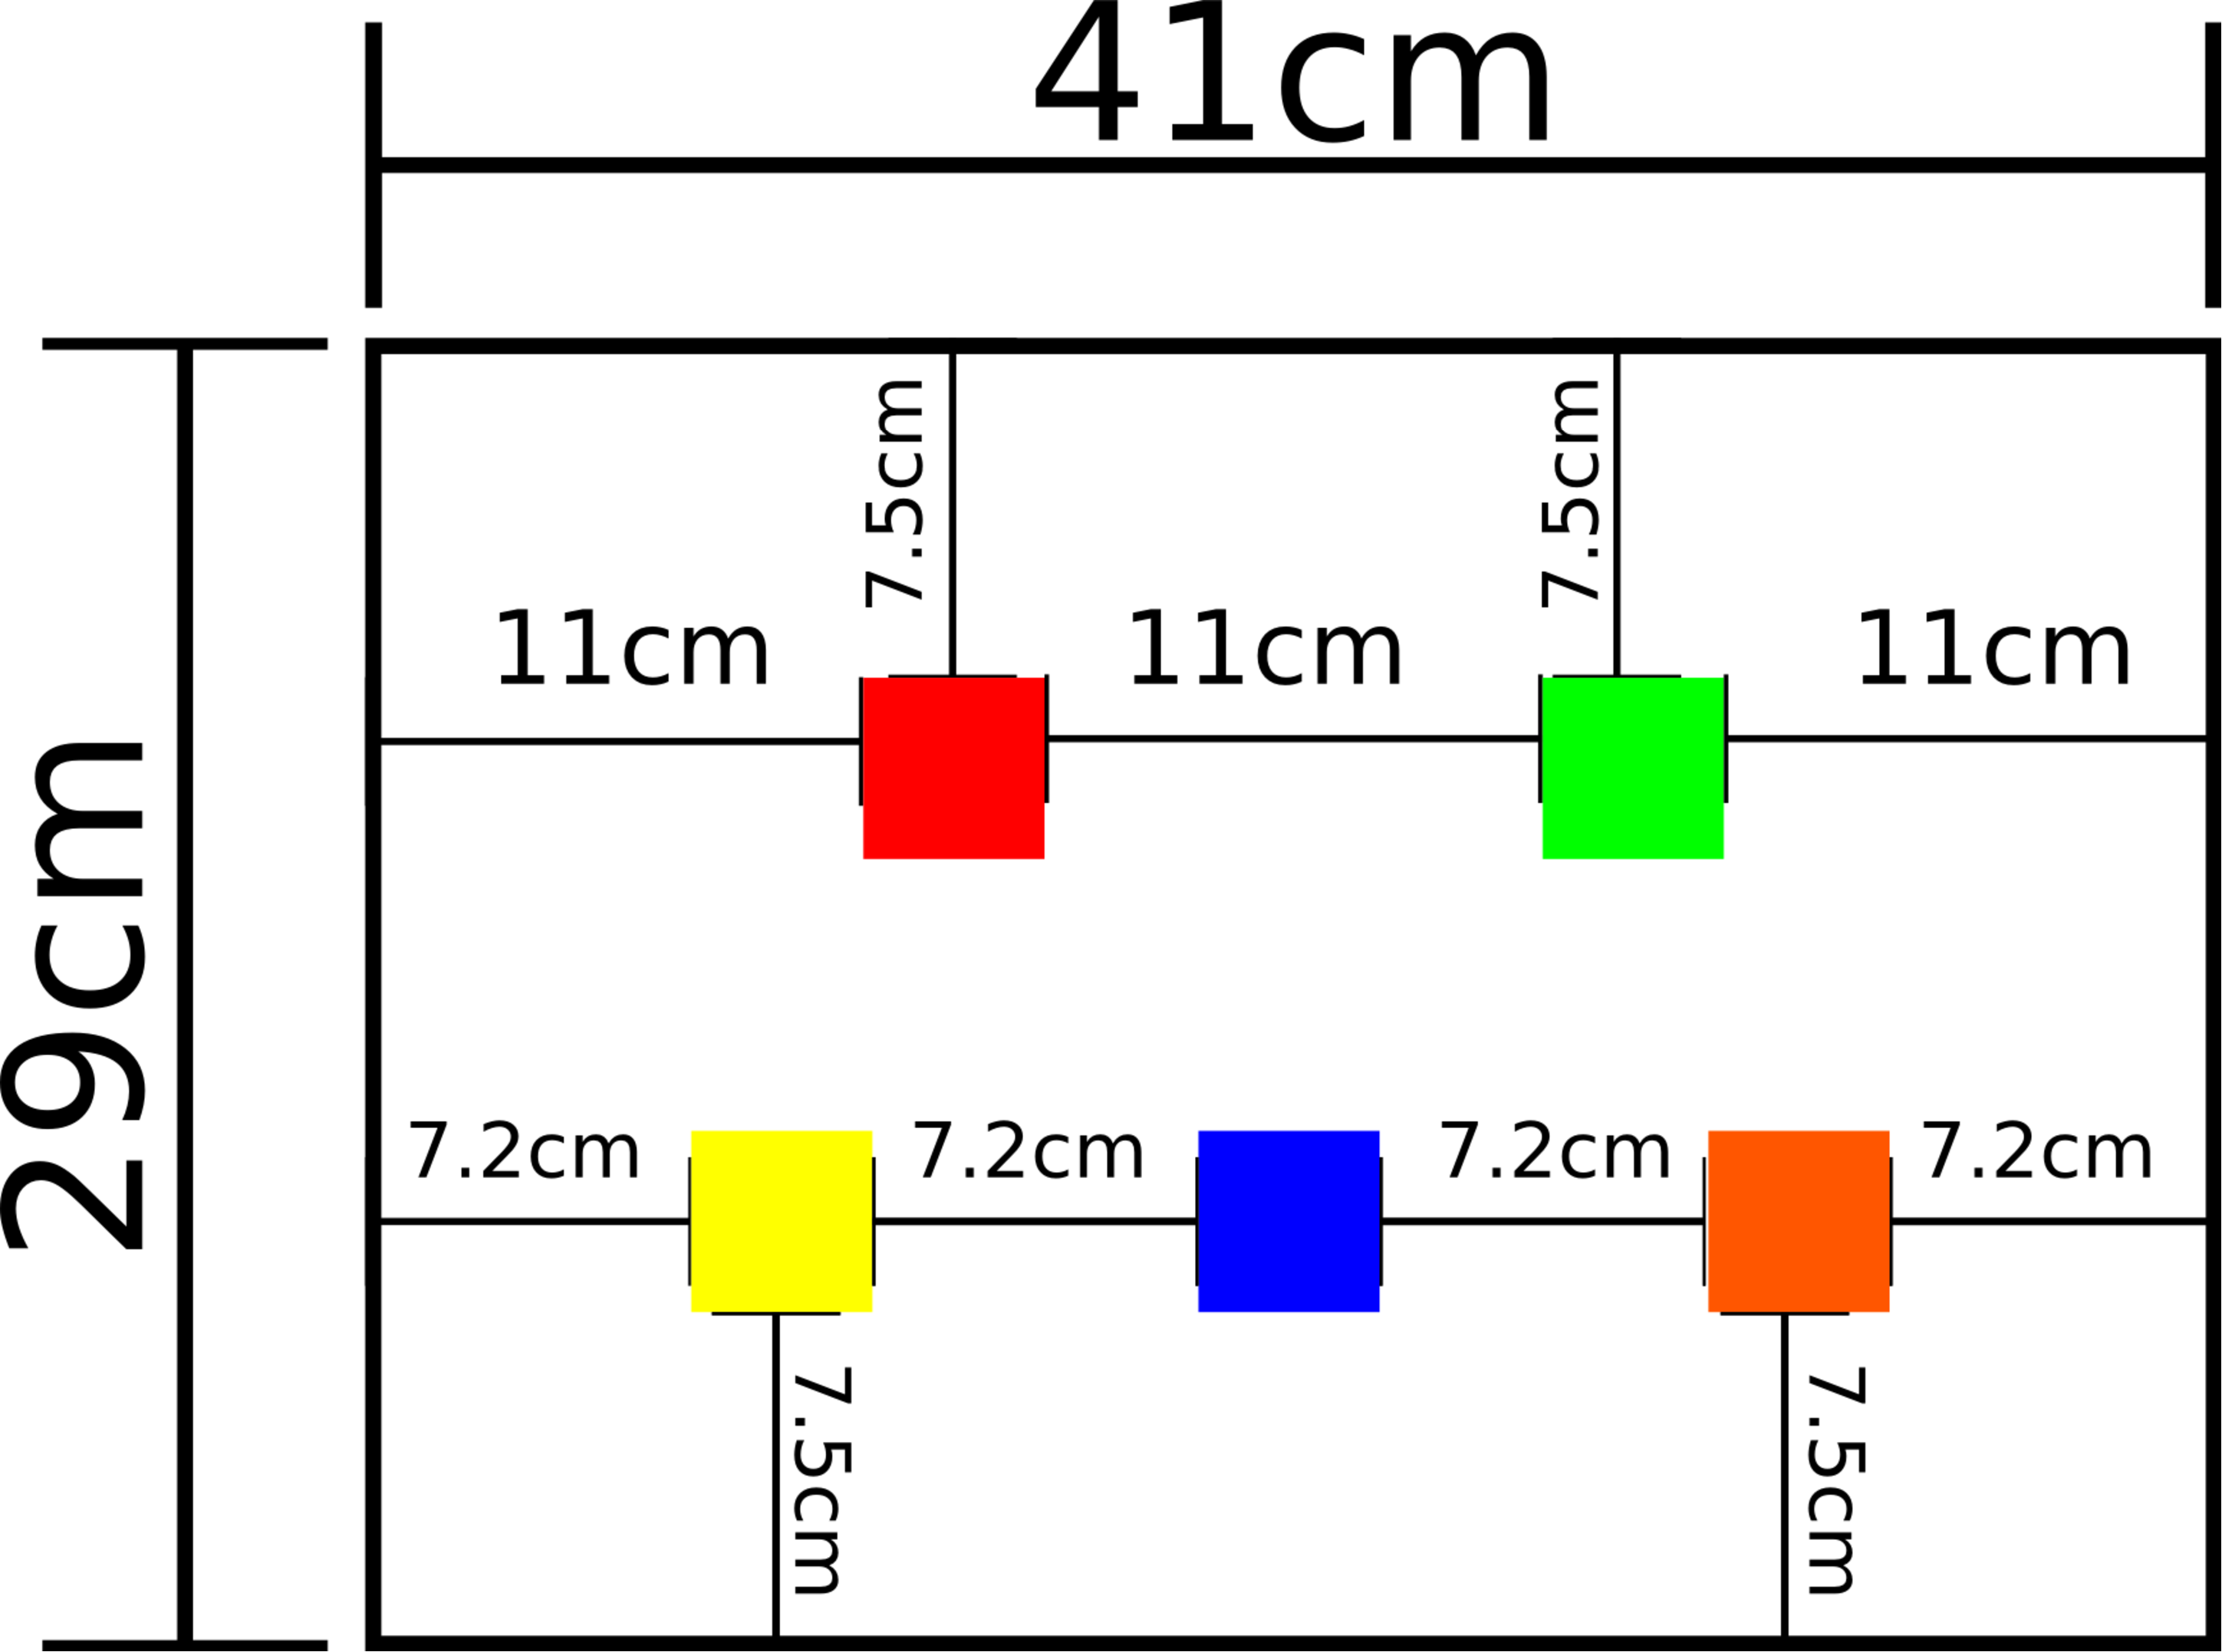
\includegraphics[width=\textwidth]{disposicaoparte.pdf}
\caption{Disposição de cada parte quanto as cores}
\label{fig:figure1}
\end{minipage}
\hspace{0.5cm}
\begin{minipage}[b]{0.45\linewidth}
\centering
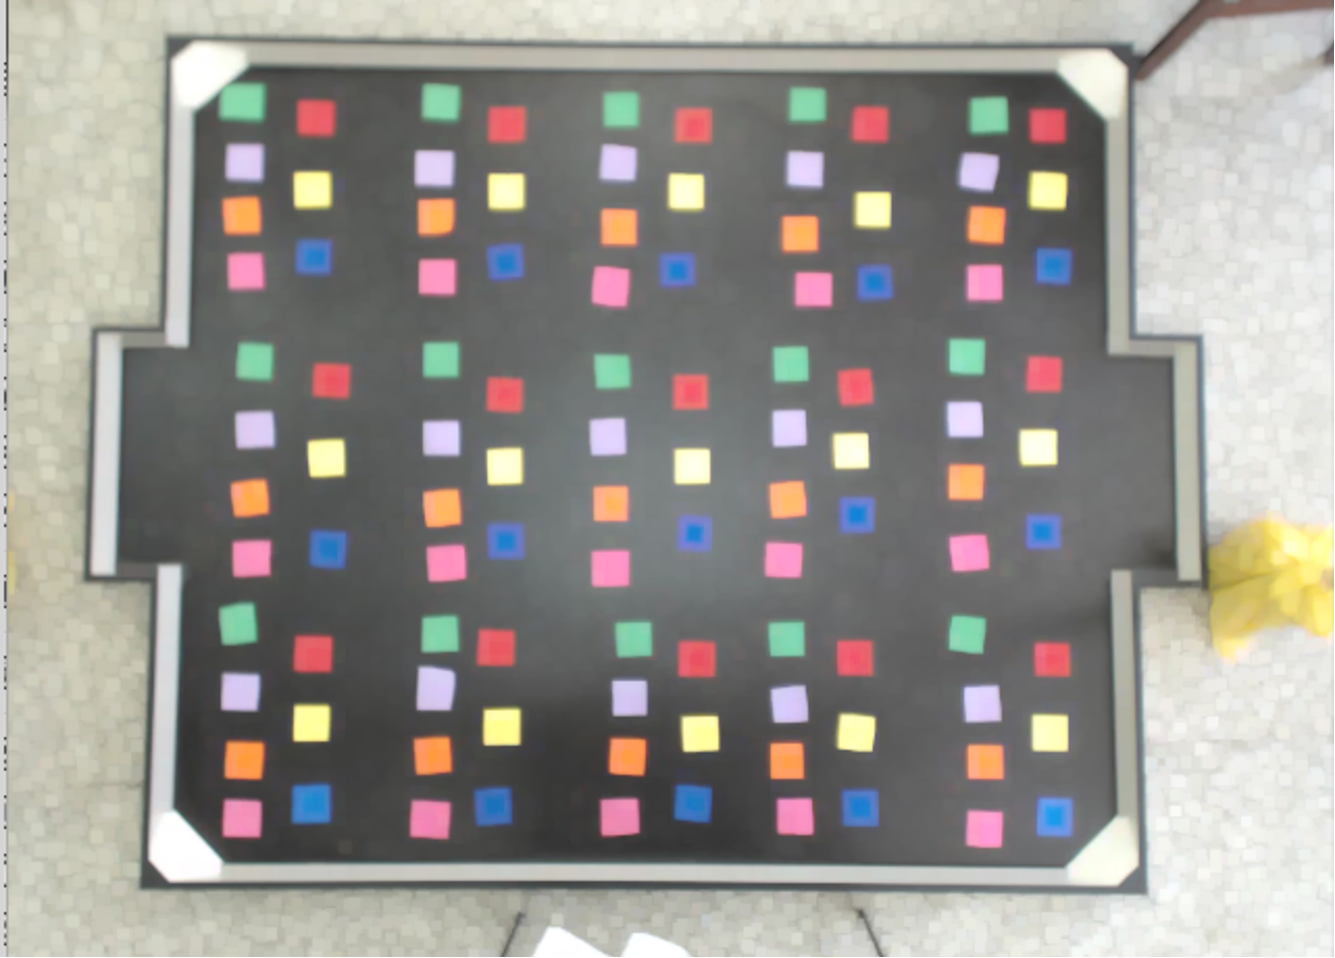
\includegraphics[width=\textwidth]{/testes/campofundo.pdf}
\caption{Campo após terem sido dispostas as cores}
\label{fig:figure2}
\end{minipage}
\end{figure}

\subsection{Cores Comuns}
\subsubsection{Amarelo}
	\begin{figure}[H]
		\centering
		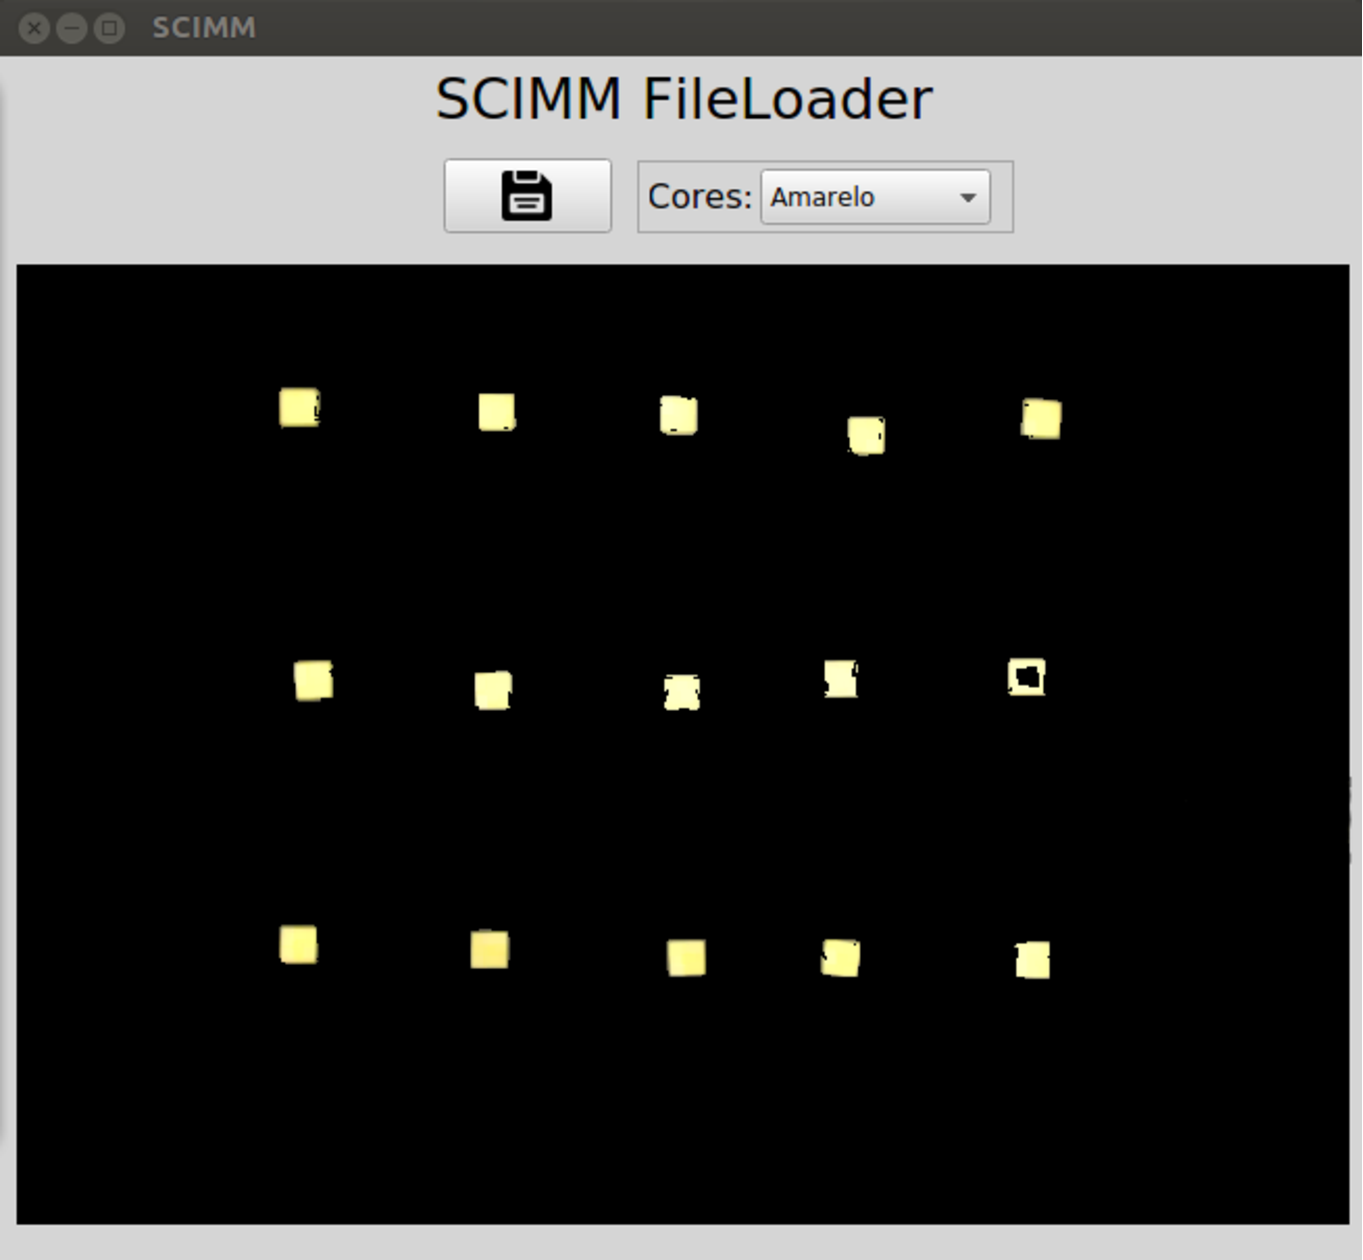
\includegraphics[width=0.5\textwidth]{/testes/amarelo.pdf}
		\caption{Imagem somente com os objetos dentro do intervalo do valor da cor amarela}
		\label{disposicaoparte}
	\end{figure}
	
	Dentre os objetos da cor amarela o sistema encontrou quatorze deles completamente e apenas um, que devido a luminosidade implicada em seu centro deixando a tonalidade muito perto do branco, não totalmente preenchido.
	
	\begin{table}[H]
\centering
\begin{tabular}{l|c|c}
Tipo de Objeto & Quantidade & \%  \\% Note a separação de col. e a quebra de linhas
\hline                               % para uma linha horizontal
Objetos Completos & 14 & 93,33 \\
\hline 
Objetos Com Falha de Preenchimento & 1 & 6,66 \\
\hline 
Objetos Com Diminuição de Contorno & 0 &\\
\hline 
Objetos Extrapolados & 0 &\\
\hline 
Objetos Com Diminuição de Área &  0 &\\
\hline 
Objetos Com Falhas Críticas & 0 &\\
\hline 
\end{tabular}
\caption{Categorização Dos Objetos}
\end{table}

Dentre as classficações dos objetos as que  \textit{Objetos Com Falhas Críticas} e \textit{Objetos Com Falha de Preenchimento} que juntos somam 6,66\% dos objetos.

\subsubsection{Azul}
	\begin{figure}[H]
		\centering
		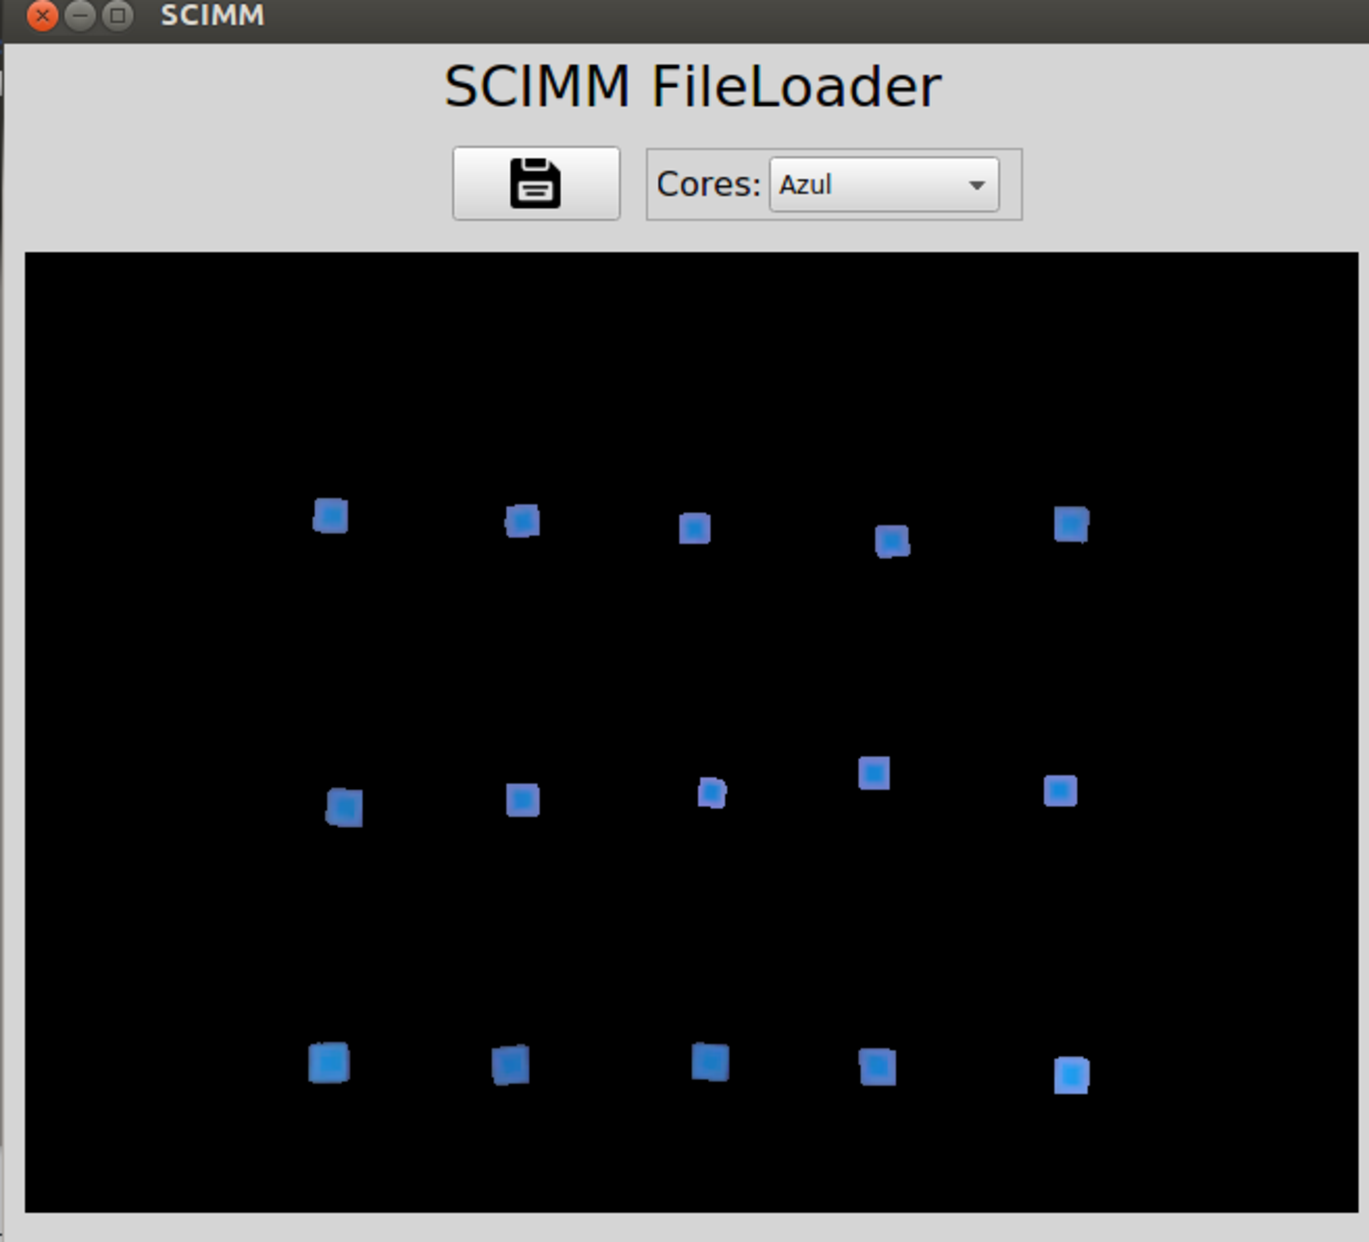
\includegraphics[width=0.5\textwidth]{/testes/azul.pdf}
		\caption{Imagem somente com os objetos dentro do intervalo do valor da cor azul}
		\label{disposicaoparte}
	\end{figure}

Os objetos da cor azul foram os que obtiveram os melhores resultados, os quinze objetos foram encontrados de forma preenchida.	Apesar dos quinze estarem totalmente preenchidos um dos objetos apresentou um tamanho reduzido aos demais devido ao fato de sua borda que não ter sido totamente detectada.

\begin{table}[h]
\centering
\begin{tabular}{l|c|c}
Tipo de Objeto & Quantidade & \% \\ % Note a separação de col. e a quebra de linhas
\hline                               % para uma linha horizontal
Objetos Completos & 14 & 93,33 \\
\hline 
Objetos Com Falha de Preenchimento & 0\\
\hline 
Objetos Com Diminuição de Contorno &  1 & 6,66
\\
\hline 
Objetos Extrapolados &  0\\
\hline 
Objetos Com Diminuição de Área & 0 \\
\hline 
Objetos Com Falhas Críticas & 0 \\
\hline 
\end{tabular}
\caption{Categorização Dos Objetos}
\end{table}

\subsubsection{Verde}
\begin{figure}[H]
		\centering
		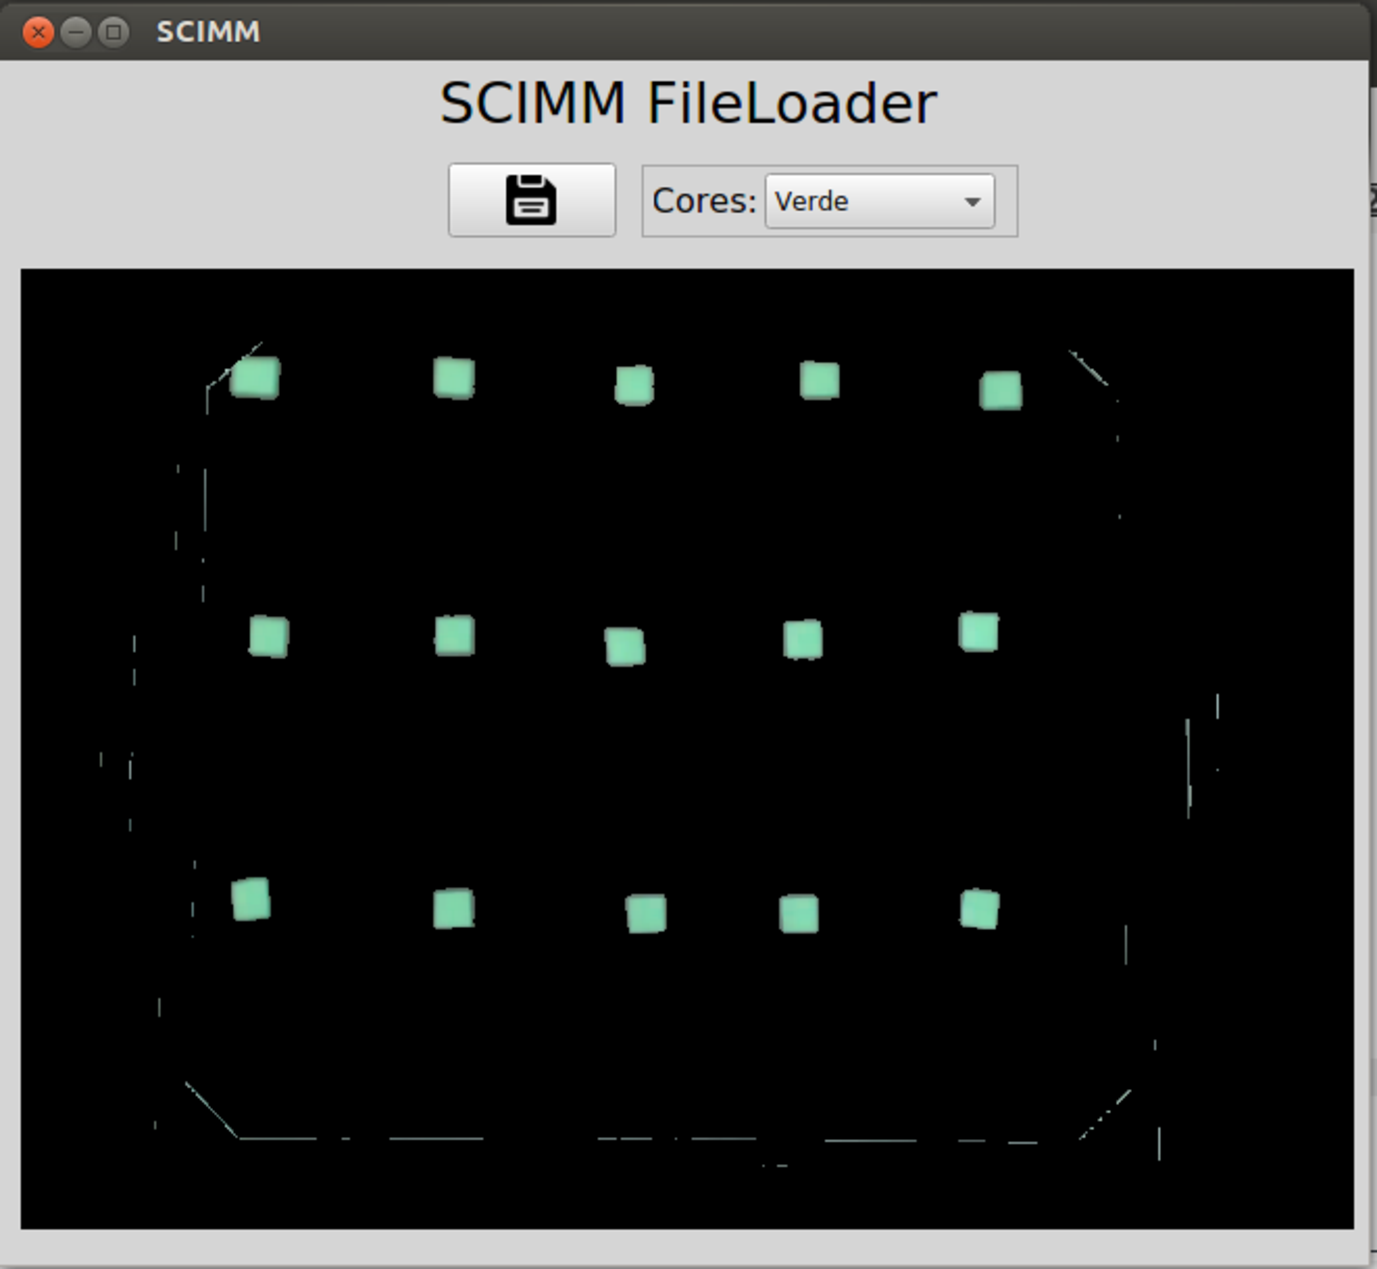
\includegraphics[width=0.5\textwidth]{/testes/verde.pdf}
		\caption{Imagem somente com os objetos dentro do intervalo do valor da cor verde}
		\label{disposicaoparte}
	\end{figure}

Os objetos da cor verde foram satisfatoriamente encontrados, com seu preenchimento total e não havendo perda de área devido a qualquer interferência de luz em sua borda.	
	
\begin{table}[h]
\centering
\begin{tabular}{l|c|c}
Tipo de Objeto & Quantidade & \% \\ % Note a separação de col. e a quebra de linhas
\hline                               % para uma linha horizontal
Objetos Completos &  15 &100 \\
\hline 
Objetos Com Falha de Preenchimento & 0\\
\hline 
Objetos Com Diminuição de Contorno &  0\\
\hline 
Objetos Extrapolados & 0 \\
\hline 
Objetos Com Diminuição de Área &  0 \\
\hline 
Objetos Com Falhas Críticas & 0 \\
\hline 
\end{tabular}
\caption{Categorização Dos Objetos}
\end{table}	
\subsubsection{Rosa}
	
	\begin{figure}[H]
		\centering
		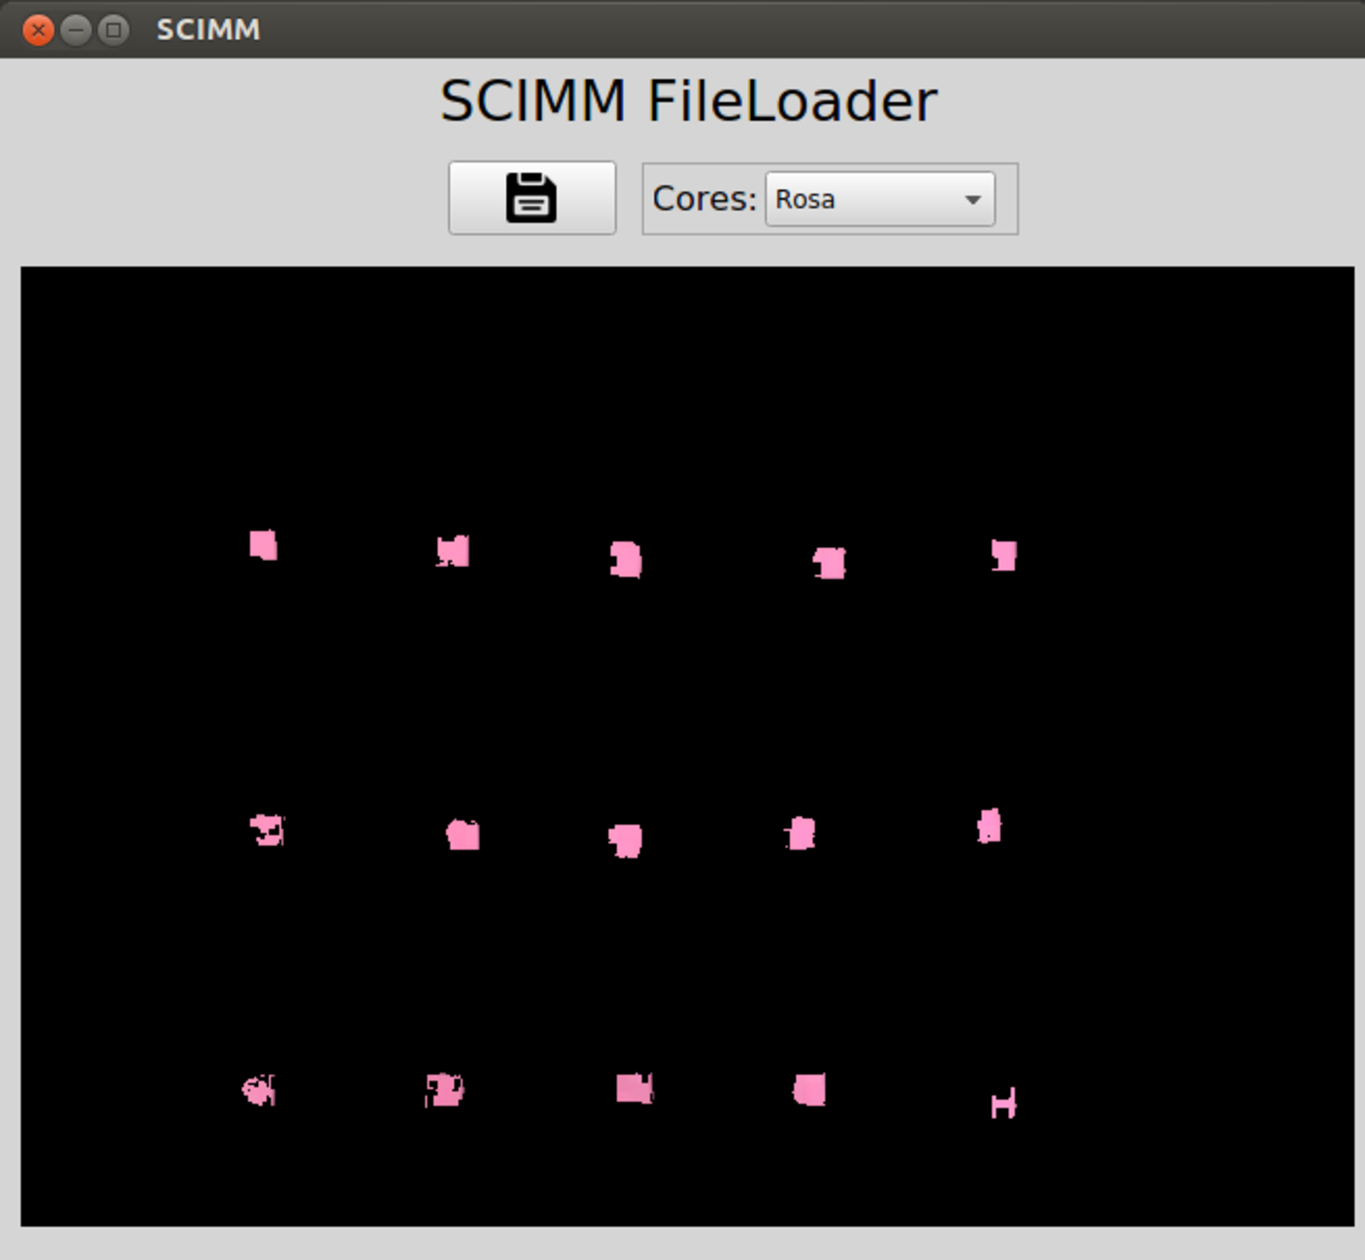
\includegraphics[width=0.5\textwidth]{/testes/rosa.pdf}
		\caption{Imagem somente com os objetos dentro do intervalo do valor da cor rosa}
		\label{disposicaoparte}
	\end{figure}
	
Dentre os objetos rosa detectados, quatro obtiveram falhas em sua detecção, falhas de preenchimento e diminuição de borda, estes podem ser desconsiderados dos objetos. Dentro os outros onze: três foram detectados sem falhas de preenchimentos apenas com diminuição de sua área para aproximadamente metade da área real do objeto; os outros oito foram encontrados apesas com diminuição de área devido a diminuição de borda.
	
	\begin{table}[h]
\centering
\begin{tabular}{l|c|c}
Tipo de Objeto & Quantidade  & \% \\ % Note a separação de col. e a quebra de linhas
\hline                               % para uma linha horizontal
Objetos Completos &  0\\
\hline 
Objetos Com Falha de Preenchimento & 0\\
\hline 
Objetos Com Diminuição de Contorno & 8& 53,33
 \\
\hline 
Objetos Extrapolados & 0 \\
\hline 
Objetos Com Diminuição de Área & 3 & 20\\
\hline 
Objetos Com Falhas Críticas & 4 & 26,66 \\
\hline 
\end{tabular}
\caption{Categorização Dos Objetos}
\end{table}

Dentre as classficações dos objetos as que  \textit{Objetos Com Falhas Críticas} e \textit{Objetos Com Falha de Preenchimento} que juntos somam 26,66\% dos objetos. Apesar de ser um numero não tão baixo, a cor rosa não é uma cor que a equipe Cedro costuma usar em seus jogos, sendo assim, essa taxa de erro não influencia na eficienca do sistema.
\subsubsection{Roxo}
\begin{figure}[H]
		\centering
		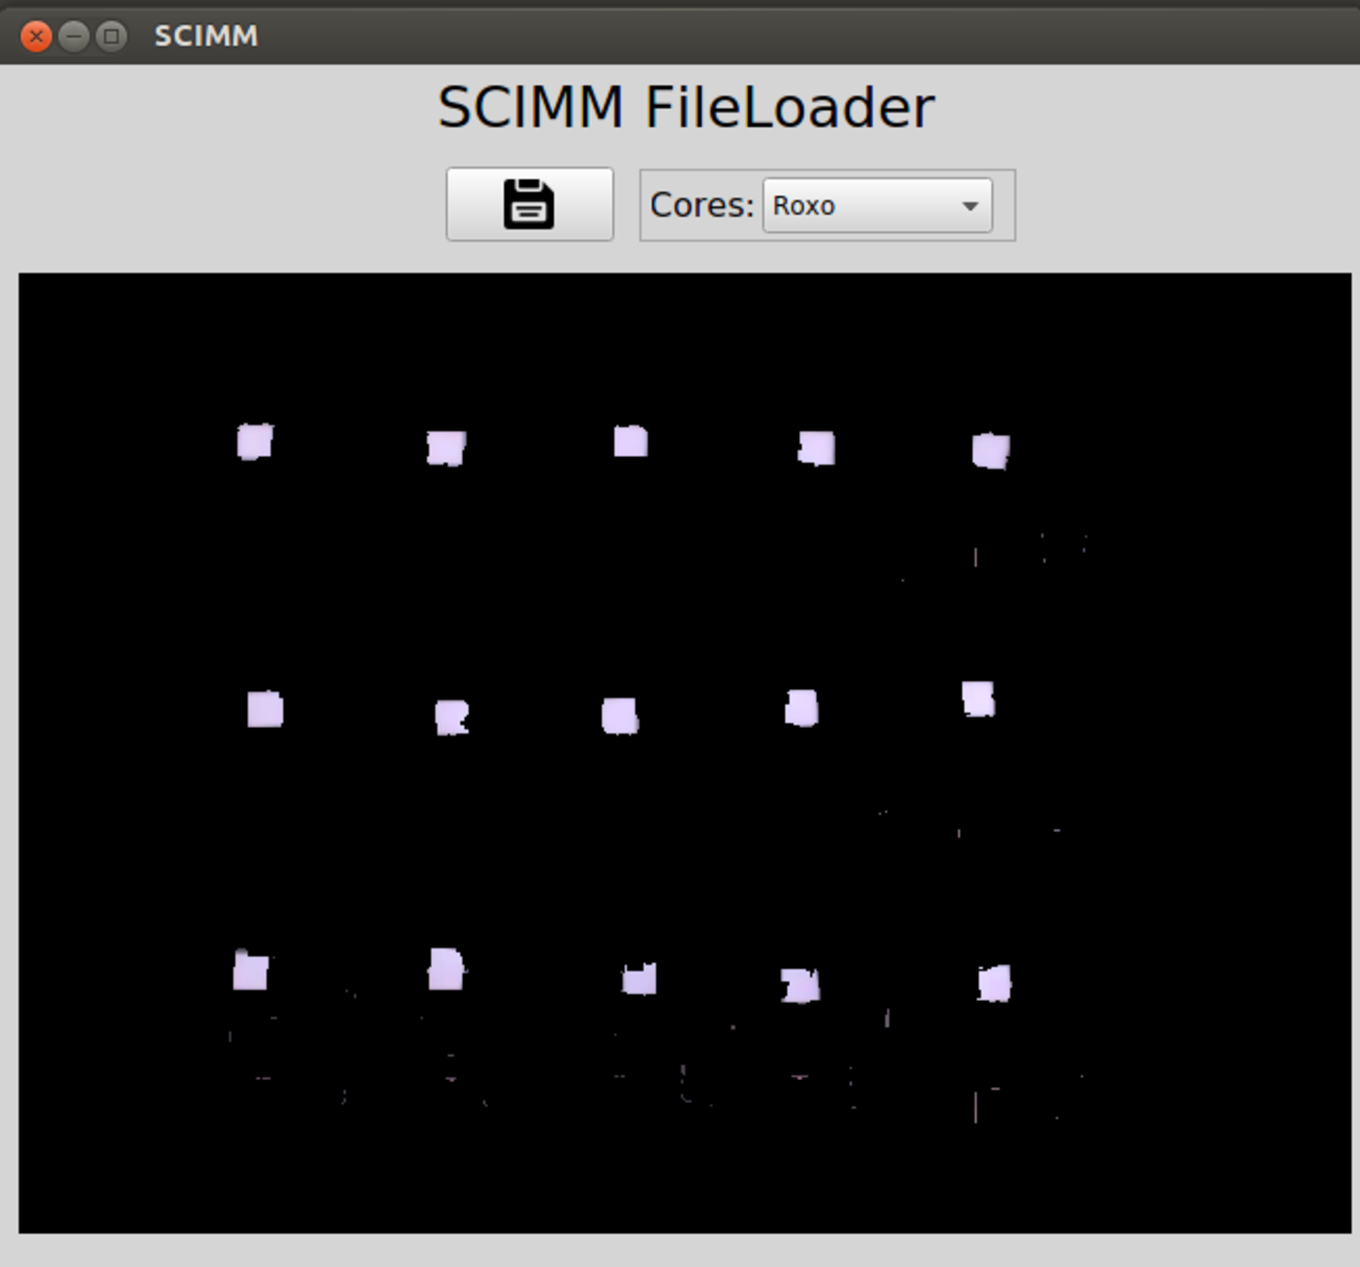
\includegraphics[width=0.5\textwidth]{/testes/roxo.pdf}
		\caption{Imagem somente com os objetos dentro do intervalo do valor da cor roxo}
		\label{disposicaoparte}
	\end{figure}

Todos os objetos roxos dispostos no campo foram encontrados pelo intervalo da cor. Dentre os quinze, quatro não apresentaram problema algum e foram completamente detectados; oito possuiram diminiução em seu contorno e três diminuição em sua área relativa.
\begin{table}[h]
\centering
\begin{tabular}{l|c|c}
Tipo de Objeto & Quantidade  & \% \\ % Note a separação de col. e a quebra de linhas
\hline                               % para uma linha horizontal
Objetos Completos &  4 & 26,66\\
\hline 
Objetos Com Falha de Preenchimento & 0 \\
\hline 
Objetos Com Diminuição de Contorno &  8 & 53,33\\
\hline 
Objetos Extrapolados & 0 \\
\hline 
Objetos Com Diminuição de Área & 3 & 20\\
\hline 
Objetos Com Falhas Críticas & 0 \\
\hline 
\end{tabular}
\caption{Categorização Dos Objetos}
\end{table}
	
\subsection{Cores Com Problemas Conhecidos}
Cores como Vermelho e Laranja possuem o problema de por vezes, devido a interferencia externas, se assemelharem a outras. Este problemas ja são de conhecimento da área.
	
	
\subsubsection{Vermelho}
	\begin{figure}[H]
		\centering
		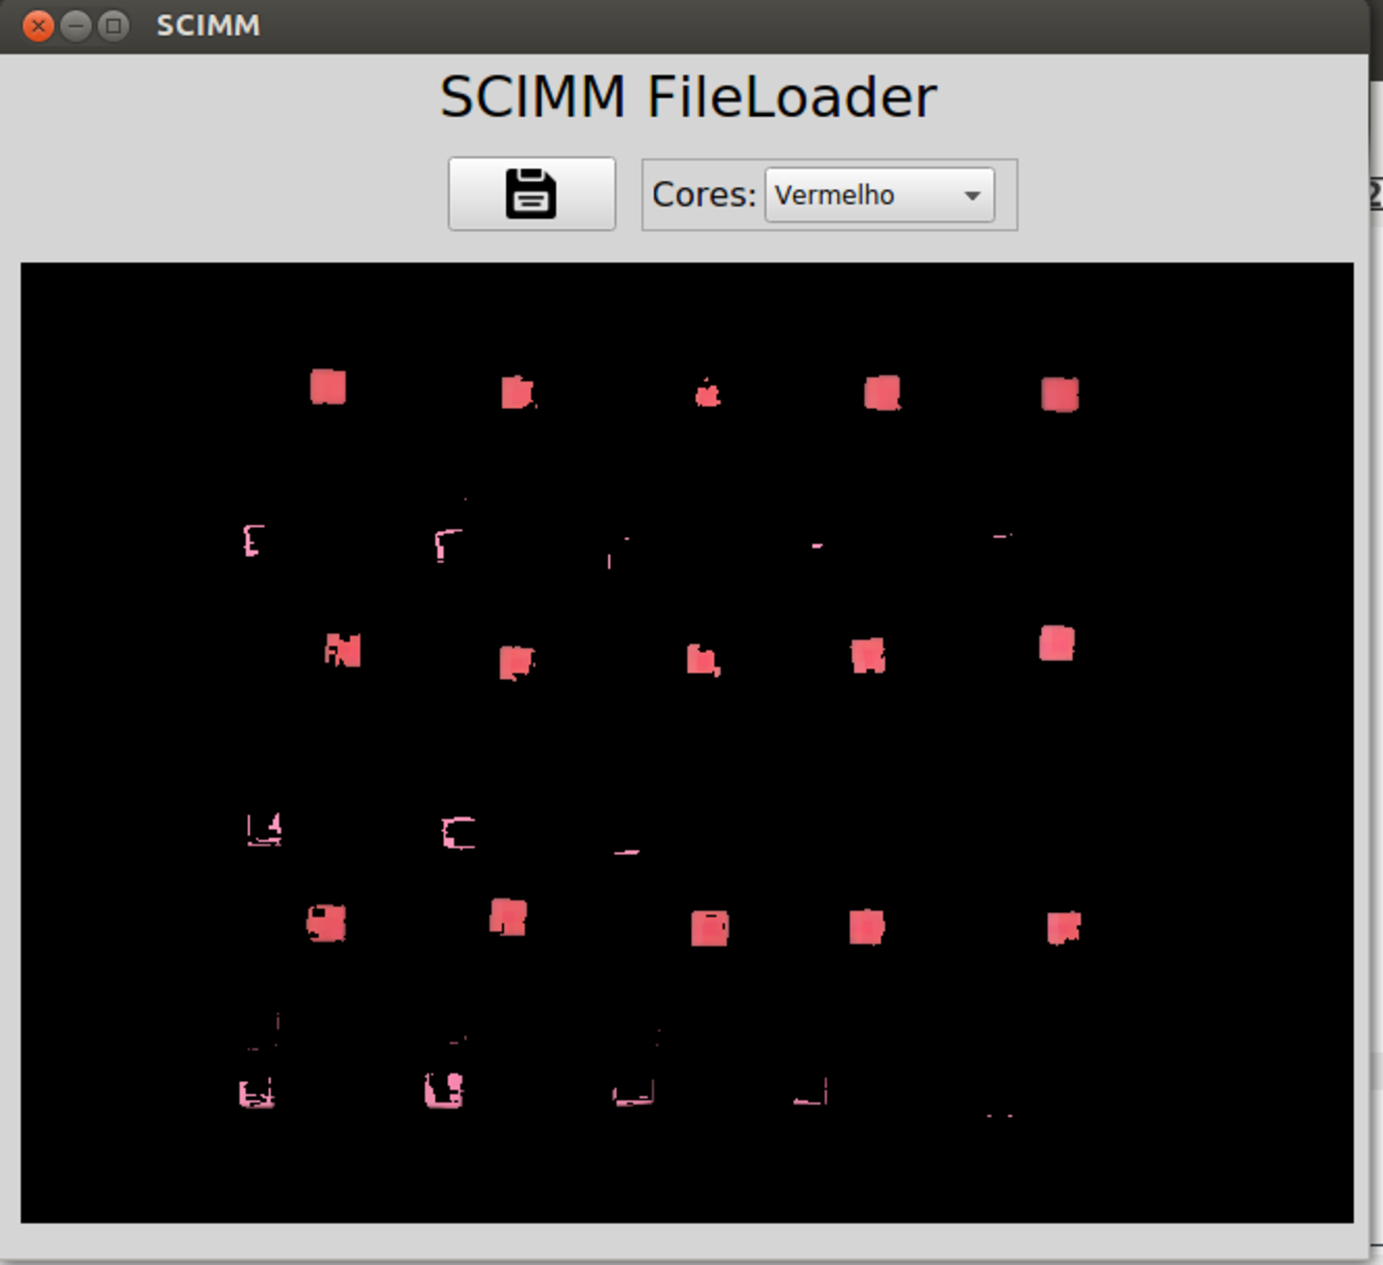
\includegraphics[width=0.5\textwidth]{/testes/vermelho.pdf}
		\caption{Imagem somente com os objetos dentro do intervalo do valor da cor vermelho}
		\label{disposicaoparte}
	\end{figure}

A cor rosa, em determinadas luminosidades pode acabar sendo semelhante a cor vermelha, por este motivo que alguns traços dos objetos rosas estão aparecendo dentro do intervalo de calibração. Porem serão ignorados, uma vez que é possível de ser feito a separação entre as das cores via software.	

	
	\begin{table}[h]
\centering
\begin{tabular}{l|c|c}
Tipo de Objeto & Quantidade  & \% \\ % Note a separação de col. e a quebra de linhas
\hline                               % para uma linha horizontal
Objetos Completos &  8 & 53,33 \\
\hline 
Objetos Com Falha de Preenchimento & 1 & 6,66 \\
\hline 
Objetos Com Diminuição de Contorno &  4 & 26,66 \\
\hline 
Objetos Extrapolados &  13 \\
\hline 
Objetos Com Diminuição de Área &  1 &6,66 \\
\hline 
Objetos Com Falhas Críticas &  1 & 6,66\\
\hline 
\end{tabular}
\caption{Categorização Dos Objetos}
\end{table}

Dentre as classficações dos objetos as que  \textit{Objetos Com Falhas Críticas} e \textit{Objetos Com Falha de Preenchimento} que juntos somam somente 13,32\% dos objetos.

\subsubsection{Laranja}
	\begin{figure}[H]
		\centering
		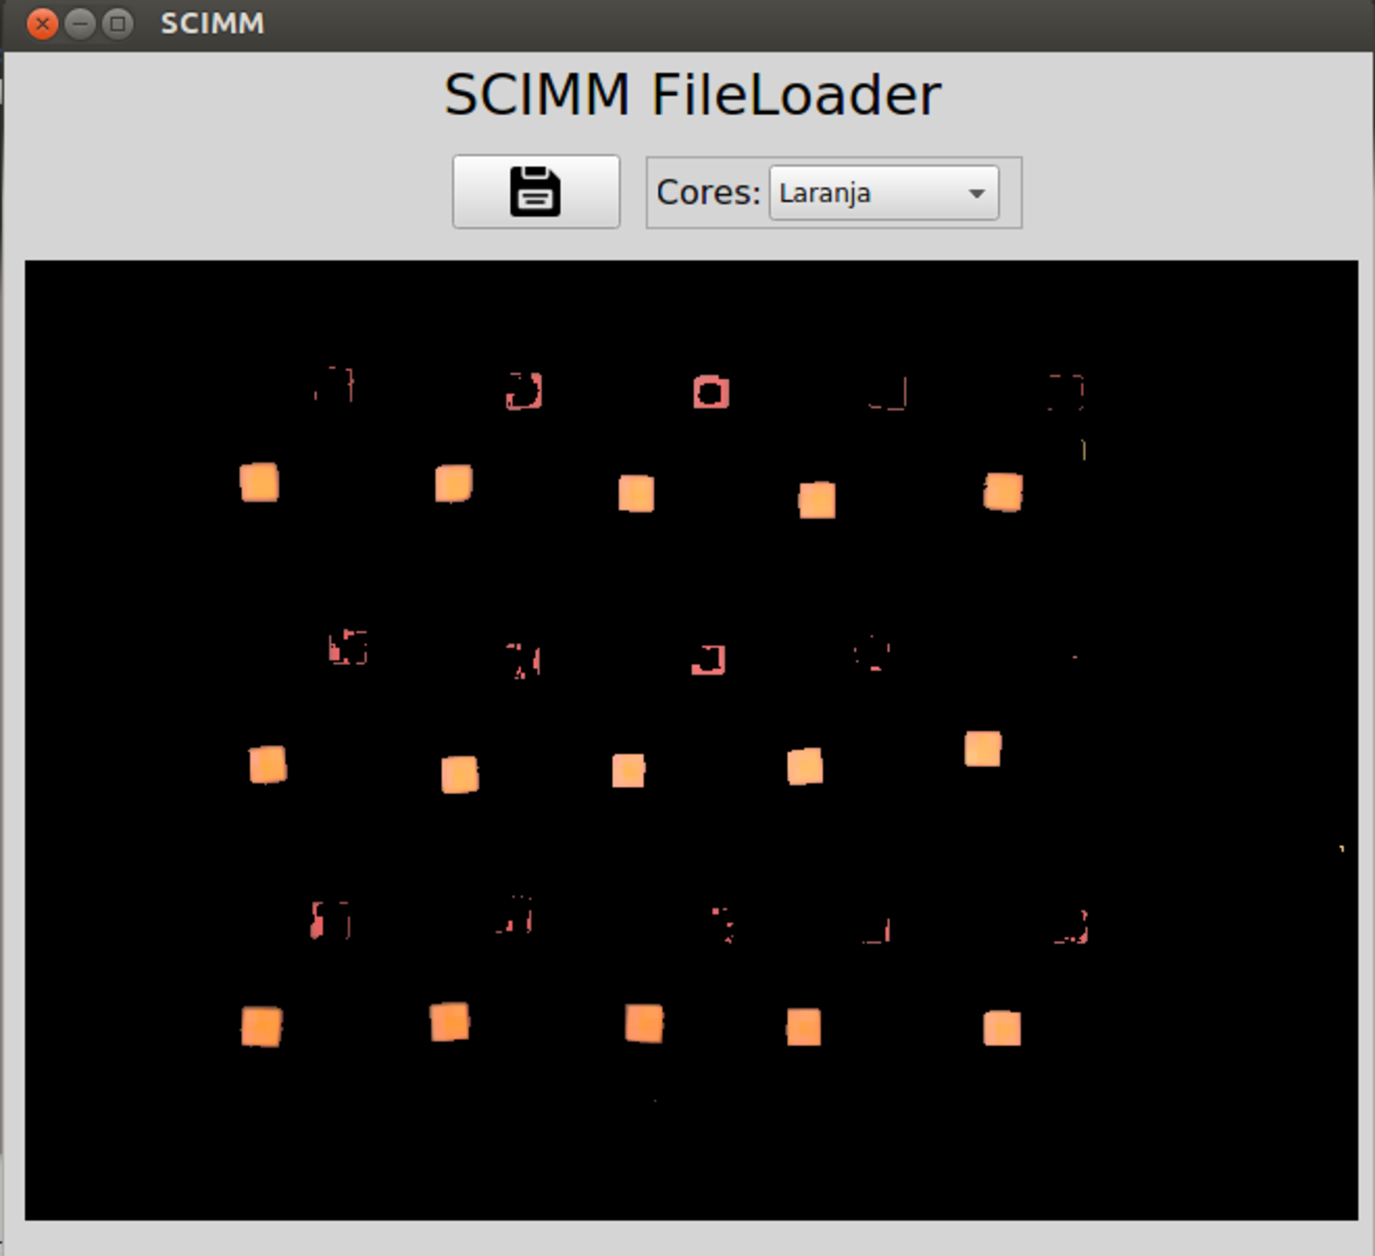
\includegraphics[width=0.5\textwidth]{/testes/laranja.pdf}
		\caption{Imagem somente com os objetos dentro do intervalo do valor da cor laranja}
		\label{disposicaoparte}
	\end{figure}
	
	Devido à um problema muito comum na área de calibração de cores, a cor laranja possui o problema de ser, por muitas vezes, semelhante a vermelha, e devido a luminosidade implicada tanto em uma quanto na outra, ambas as cores tendem a se tornarem próximas.
	Sabendo deste problema, o fato de terem sido encontrados objetos da cor vermelha dentro do intervalo de valores da cor laranja é ignorado e somente serão levados em consideração os objetos visualmente laranjas.
	Os quinze objetos da cor laranja foram encontrados com precisão. Todos possuindo seu completo preenchimento e borda.
	
\begin{table}[h]
\centering
\begin{tabular}{l|c|c}
Tipo de Objeto & Quantidade  & \% \\ % Note a separação de col. e a quebra de linhas
\hline                               % para uma linha horizontal
Objetos Completos &  15 & 100 \\
\hline 
Objetos Com Falha de Preenchimento & 0 \\
\hline 
Objetos Com Diminuição de Contorno &  0 \\
\hline 
Objetos Extrapolados & 8 \\
\hline 
Objetos Com Diminuição de Área &  0 \\
\hline 
Objetos Com Falhas Críticas & 0 \\
\hline 
\end{tabular}
\caption{Categorização Dos Objetos}
\end{table}
\newpage
\subsubsection{Totais}
De modo total estavam disposto pelo campo 105 objetos coloridos. Destes, 66,7\% dos objetos foram encontrados corretamente, 1,9\% foram encontrados com falhas de preenchimento, 20\% apresentaram perda de contorno, 6,67\% apresentaram diminuição da área e 4,76\% apresentaram falhas e faltas que prejudicaram totalmente o objeto.
	\begin{figure}[H]
		\centering
		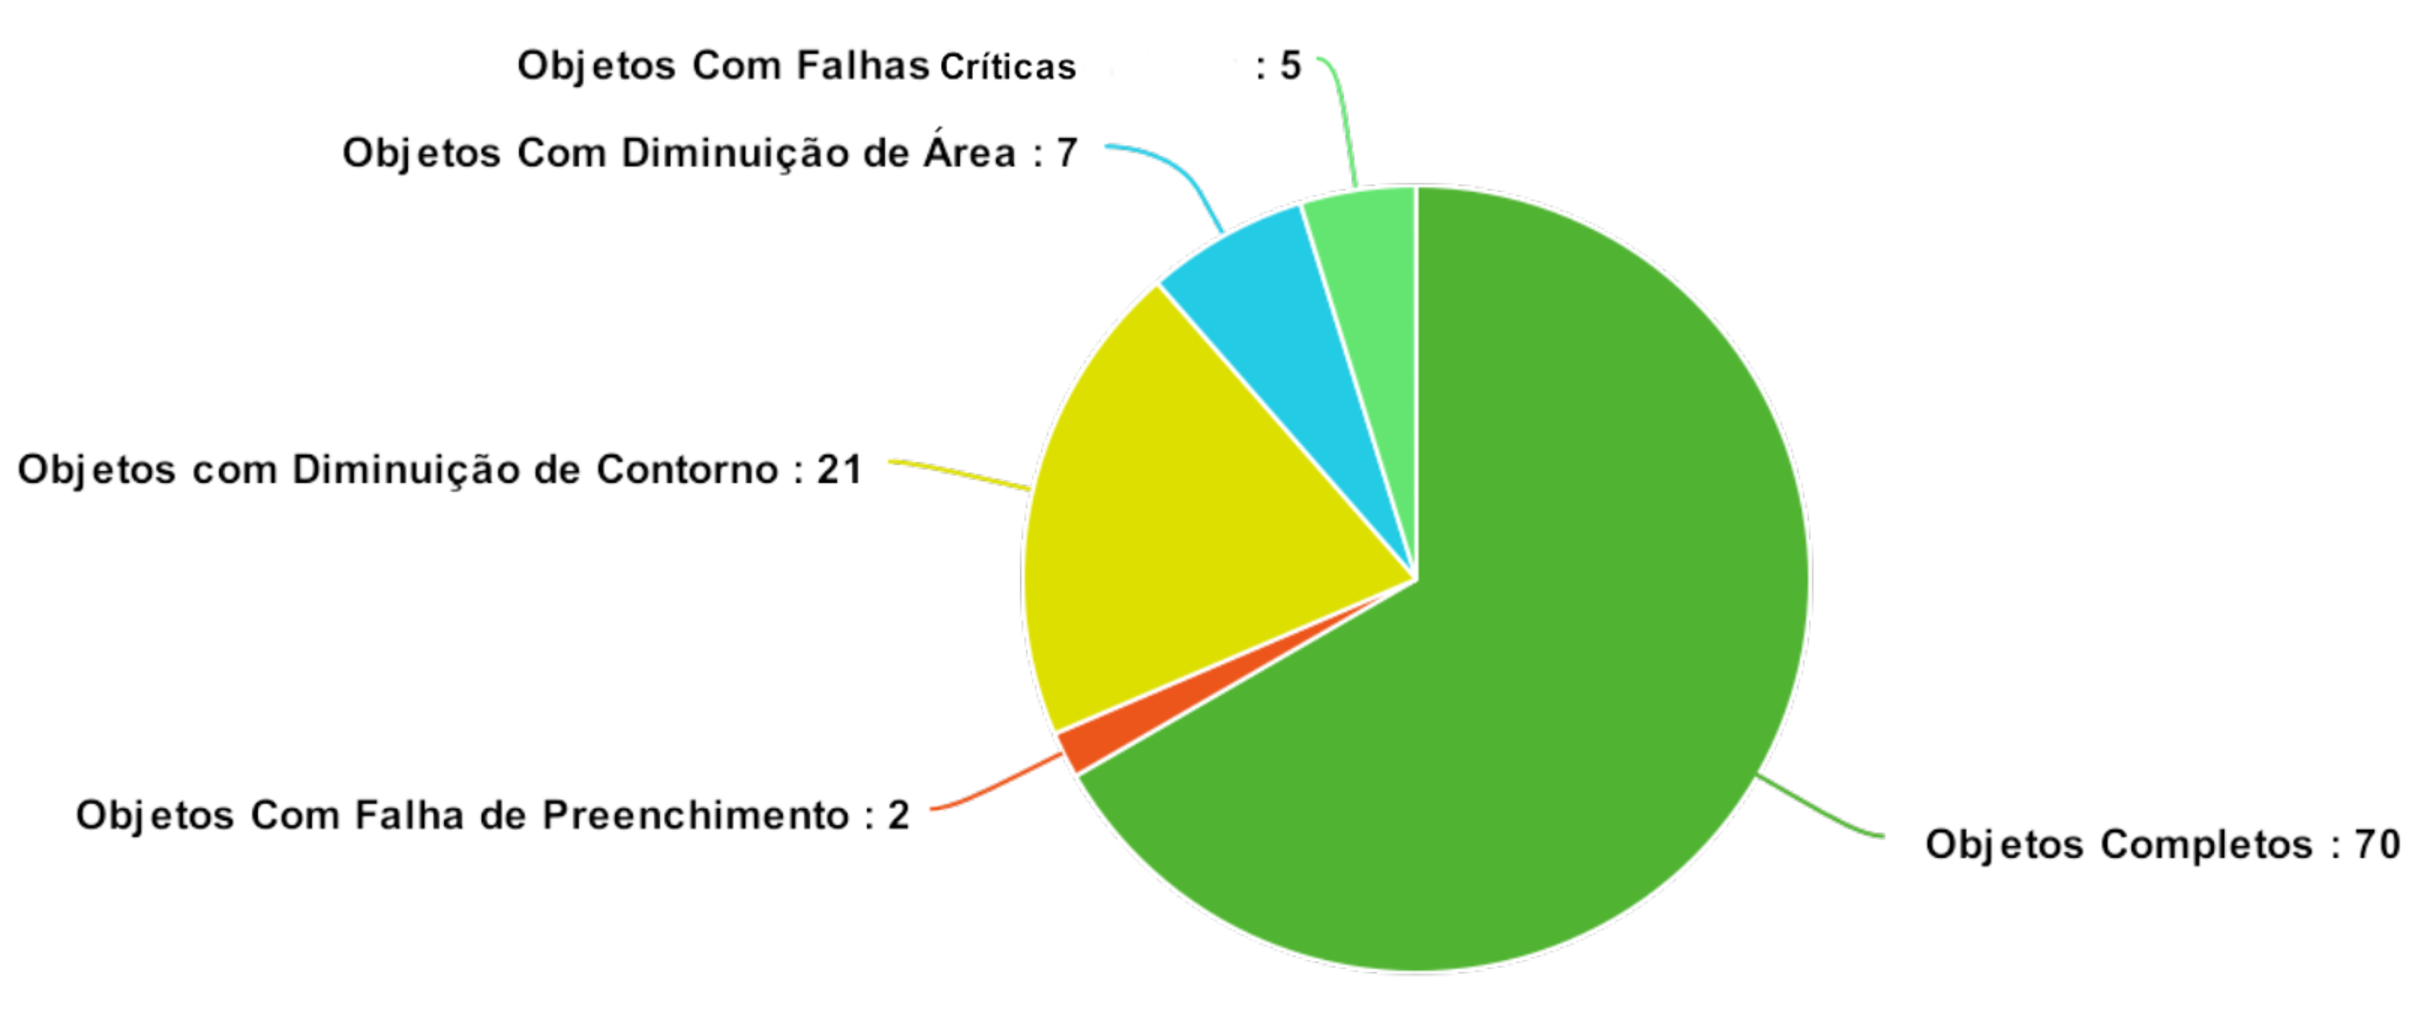
\includegraphics[width=0.8\textwidth]{/testes/graficotestes.pdf}
		\caption{Gráfico de análise do resultado dos testes}
		\label{disposicaoparte}
	\end{figure}
	
	
	Sabendo destes valores, os que podem ser considerados críticos na detecção de objetos por meio da sua cor são \textit{Objetos Com Falhas Críticas} e \textit{Objetos Com Falha de Preenchimento} que juntos somam 6,67\% dos objetos.